\chapter{Tesztek laborkörülmények között}

\section{A kísérleti rendszer}
Az elméleti eredmények validálásához elkészítettem egy szoba kicsinyített modelljét. Ez egy kartondobozban kapott helyet. A doboz hőtároló képessége elég csekély, ezért extra hőtároló tömegeket helyeztem bele, OSB falapot és egy elektromos kályhából vett samott téglát.
A fűtési teljesítményt halogén izzókkal juttattuk a rendszerbe. Ezek teljesítménye szabályozható, így ez a bemenet lineáris a szelepekkel ellentétben, azaz kétszer nagyobb beavatkozójelre kétszer nagyobb teljesítmény kerül a rendszerbe.
A hőmérsékletet mérjük a dobozban és azon kívül is. Zavarásként a mérőszoba ablakát kinyitjuk, így a doboz környezeti hőmérséklete lecsökken.

\section{A Simulink konfigurálása}
A valós idejű futáshoz Simulink  Real-time szükséges. A real-time működés itt azt jelenti, hogy a szabályzót a Simulink mintavételi időnként futtatja le. Azaz ha a kísérleti rendszerre \SI{30}{\second}-es mintavételi idejű szabályzót tervezek, akkor az MPC félpercenként mintát fog venni a hőmérsékletekből és ki fog adni egy beavatkozójelet. Így a real-time ez esetben nem jelent például szigorú korlátokat a futásidőre.


%A Real-time UDP-t használom. %https://uk.mathworks.com/help/xpc/io_ref/udp-transport-protocol.html
%https://uk.mathworks.com/products/simulink-desktop-real-time.html

A szabályzó a számítógépen fog futni, és mintavételi időnként a jelenlegi hőmérsékletet beolvassa, az MPC-t lefuttatja, a beavatkozó jeleket pedig elküldi a beágyazott számítógépnek.

\begin{figure}
	\centering
	\begin{tikzpicture}[>=stealth,
  		%inner/.style={draw,fill=blue!5,thick,inner sep=3pt,minimum width=8em},
		%outer/.style={draw=gray,dashed,fill=green!1,thick,inner sep=5pt}
		outer/.style={draw=gray,dashed,thick,inner sep=5pt}
		]
	\node[rectangle, minimum height=0.8cm,minimum width=2cm] (ghostDist) at (0,-2) {Zavarás};
	\node[draw,rectangle, minimum height=2cm,minimum width=6cm] (Numeric) at (2.3,3.5) {\parbox{2cm}{\centering MPC szabályzás}};
	\node[draw,outer,rectangle, minimum height=4cm,minimum width=8cm,
			label={[label distance=-0.75cm]120:Matlab Simulink}] (keret) at (2.3,3.5) {};
			

	%\node[draw,rectangle, minimum height=2cm,minimum width=5.5cm] (Simsc) at (9,2.5) {\parbox{2cm}{\centering fűtési rendszer Simscape}};
	\node[draw,rectangle, minimum height=1.5cm,minimum width=5cm] (heat) at (5,0) {\parbox{2cm}{\centering vezérlés és fűtőtest (lámpa)}};
	\node[draw,rectangle, minimum height=1.5cm,minimum width=3cm] (house) at (0,0) {ház};
	\draw[->] (ghostDist.90) --  (house.270) node[above]{$T_e$};  %node[above left]{$\alpha_{radiator}$}; 
	\draw[->] (ghostDist.180) -| ++(-2.5,0)  |-  (Numeric.168) node[right]{MD} ;
	
	%\draw[->] (ctr.191) node[right]{${u_{2}}$} -| ++(-1.7,1.3)|-  (Numeric.172) node[right]{$\alpha_{floor}$};  %node[above left]{$\alpha_{radiator}$}; 
	\draw[->] (ctr.169) node[right]{${T_{i}}$}-| ++(-1,0.8)  |-  (Numeric.188) node[right]{MO} ;
	
	%\draw[->] (d.0) node[left]{heat [W]} ->  ++(3,0) ->  (house.180);
	\draw [->] (Numeric.0) node[left]{MV} -| ++(3,-2.5)  |- (heat.0) node[left]{${PWM_{\%}}$}; %++(1.5cm,0) -- (2cm,0pt) -- (2.5cm,10pt);
	
	\draw[->] (heat.180)  node[right]{$Q_{ki}$} -- (ctr.0) ;
	%\draw[->] (d.20) -| ++(1,-1) |- (y.350);
	
	%\path 
	%(d.150)	 edge[<->] 	node[anchor=north,above]{valvePercent}	(y.270);
	
	\end{tikzpicture}

	\caption{A szimulációban szereplő elemek kapcsolata}
	\label{controlloop}
\end{figure}

%\begin{tikzpicture}[>=stealth,remember picture]
%\node[draw,rectangle,inner sep=0.5cm] (y) at (0,0) {$A$};
%\node[draw] (d) at (0,2) {%
%%	\begin{tikzpicture}[remember picture]
%%	\matrix [matrix of math nodes] (mat)
%%	{
%%		B & \phantom{C}   \\
%%		\phantom{B} & C \\
%%	};
%%	\end{tikzpicture}
%%};
%%\draw[->,shorten >= 6pt] (y.west) -| ++(-1,1) |- (mat-1-1);
%%\draw[->,shorten >= 6pt] (y.west) -| ++(-0.8,1) |- (mat-2-1);
%%\draw[->] ($(mat-2-2)+(14pt,0)$) -| ++(0.8,-1) |- (y.east);
%%\draw[->] ($(mat-1-2)+(14pt,0)$) -| ++(1,-1) |- (y.east);
%\end{tikzpicture}




% 3600001117-es ID-jű, Raspberry Pi, IP címe fixen 192.168.0.108, 54321-es port.

%A PI SPI-n küld a rádióadónak.
%Rádiókommunikáció egyirányú.

\section{Mintavételi idő és predikciós horizont}

Az MPC paraméterezésére \textit{Agachi \cite{romanMPC_Agachi}} könyvében találhatók ajánlások. A predikciós horizontot eszerint úgy kell megválasztani, hogy az a szakasz releváns dinamikáját lefedje. Mivel a felfutási ideje a kísérleti rendszernek kb. 1 óra, ezért ezt ekkorára választottam. A predikciós horizont ajánlott nagysága 10-20 mintavétel a számítási igény csökkentése miatt (így $T_s =$ \SI{300}{\second} adódna),  viszont a mérés során gyakrabban szerettem volna látni a változásokat, a mintavételi időt 30 másodpercnek vettem.

A fentiek mellett viszont a szabályzó nem adott ki beavatkozójelet egészen egy predikciós horizontnyi ideig, azaz majdnem 1 órán keresztül\footnote{Ha 300 másodperces mintavételi időt használtam és 10 mintányi predikciós horizontot, ugyanez volt a helyzet. Ez idő alatt az MPC valószínűleg az állapotbecslőjét inicializálja.}. Az MPC képes a költségfüggvényben figyelembe venni a predikciós horizonton belül a referenciajel jövőbeli változásait (ez a \textit{Signal Previewing}), ezt kipróbáltam annak érdekében, hogy ezt a \say{holtidőt} csökkentsem, ám ellentétes hatást értem el.

A Simulink blokk viszont támogatja az MPC-nek kezdeti érték megadását. A kezdeti érték nélküli MPC-t szimulációban (azaz nem valós időben) futtattam, majd leolvastam annak belső állapotát. Az \verb|mpcstate| függvénnyel létre kellett hoznom egy objektumot, ami a Simulinkben a szabályzót inicializálja. Ehhez szükség volt a szabályzó állapotteres szakaszmodelljének\footnote{Amikor az MPC-t létrehozzuk, a szakaszmodellt a Matlab állapotteressé alakítja.} becsült állapotára, a zavarjel becsült értékére, a zaj becsült értékére (ez esetben üres vektor), a legutóbbi beavatkozójelre és egy kovarianciamátrixra (ezt nullmátrixnak vettem).

Azzal, hogy a fenti objektumban a legutóbbi beavatkozójelet maximálisnak vettem, valós idejű futás esetén, a fizikai rendszer ugrásválaszánál nem kellett kivárnom egy órát, azaz a predikciós horizontnyi időt, hanem a szabályzó rögtön maximális beavatkozójelet adott ki.

%\begin{lstlisting}[
%style=Matlab-editor,
%basicstyle=\mlttfamily,
%escapechar=`,
%]
%mpcstate05=mpcstate(mpc_labsys05,[163 81.5 11600],-0.858,[],1,zeros(4))
%MPCSTATE object with fields
%Plant: [163 81.5000 11600]
%Disturbance: -0.8580
%Noise: [1×0 double]
%LastMove: 1
%MATLAB Command Window Page 2
%Covariance: [4×4 double]
%\end{lstlisting}

\section{Szabályozótervezés az identifikált modellre}

A valós idejű méréshez használt szabályzót érdemes először szimulációban megvizsgálni. Ekkor az identifikált lineáris modell a szabályzott szakasz, a szabályzóparaméterek megváltoztatását pedig gyorsan meg lehet figyelni.



\begin{figure}[H]
	\begin{subfigure}[t]{0.32\textwidth}
		\centering
		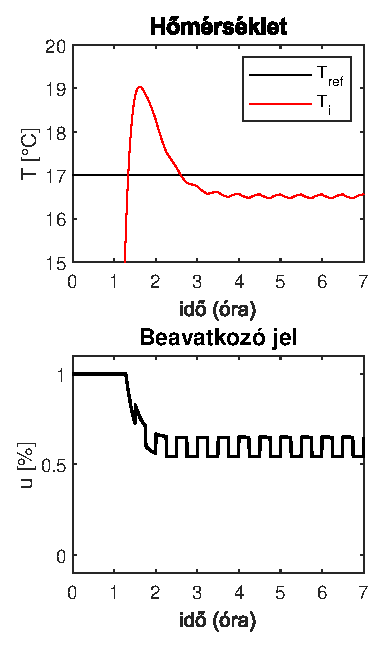
\includegraphics[width=\textwidth]{figures/realsys/mpc-wy-1}
		\caption{$w_y=1$}
		\label{fig:mpc-wy-1}
	\end{subfigure}
	~
	\begin{subfigure}[t]{0.32\textwidth}
		\centering
		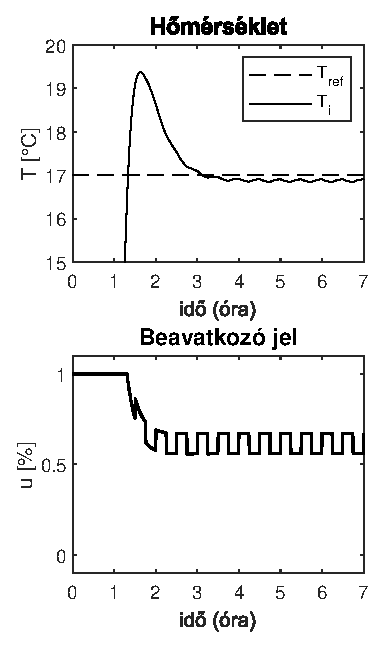
\includegraphics[width=\textwidth]{figures/realsys/mpc-wy-2}
		\caption{$w_y=2$}
		\label{fig:mpc-wy-2}
	\end{subfigure}
	~
	\begin{subfigure}[t]{0.32\textwidth}
		\centering
		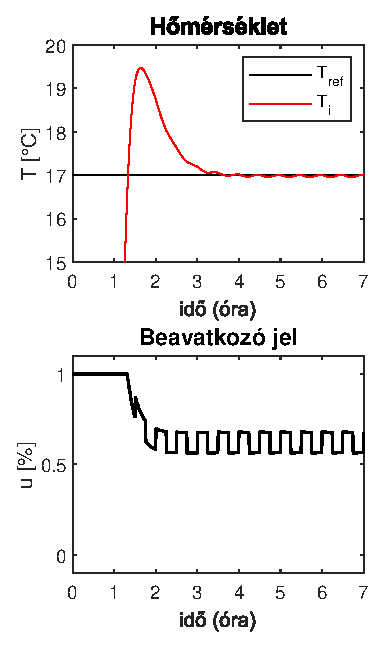
\includegraphics[width=\textwidth]{figures/realsys/mpc-wy-5}
		\caption{$w_y=5$}
		\label{fig:mpc-wy-5}
	\end{subfigure}
	\caption{MPC viselkedése különböző $w_y$ értékekre}
	\label{fig:mpc-wy}
\end{figure}



\begin{figure}[H]
\begin{subfigure}[t]{0.32\textwidth}
	\centering
	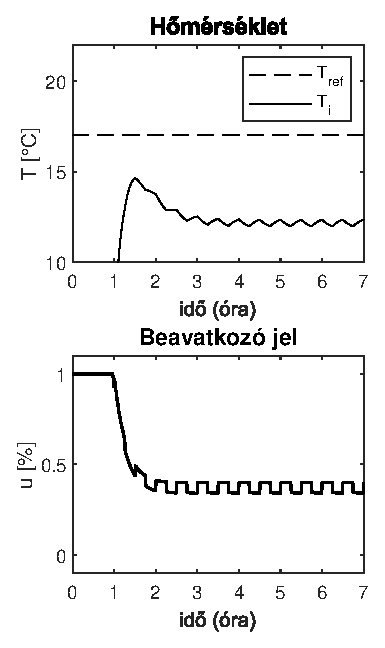
\includegraphics[width=\textwidth]{figures/realsys/mpc-wu-20}
	\caption{$w_u=20$}
	\label{fig:mpc-wu-20}
\end{subfigure}
~
\begin{subfigure}[t]{0.32\textwidth}
	\centering
	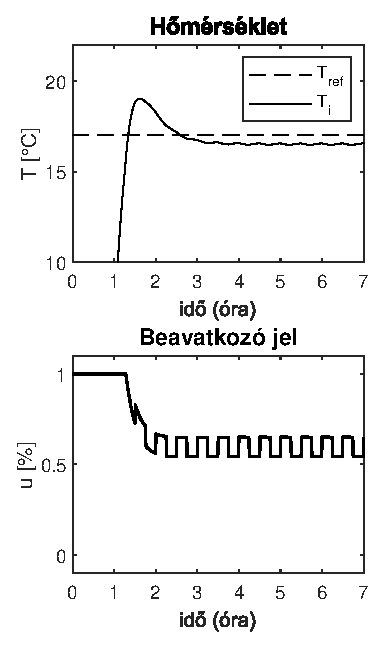
\includegraphics[width=\textwidth]{figures/realsys/mpc-wu-05}
	\caption{$w_u=5$}
	\label{fig:mpc-wu-05}
\end{subfigure}
~
\begin{subfigure}[t]{0.32\textwidth}
	\centering
	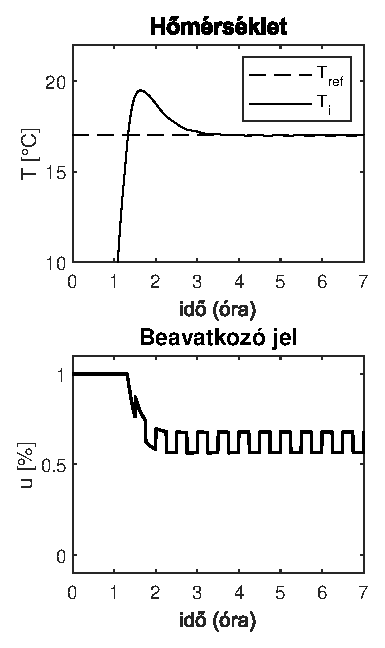
\includegraphics[width=\textwidth]{figures/realsys/mpc-wu-005}
	\caption{$w_u=0.05$}
	\label{fig:mpc-wu-005}
\end{subfigure}
\caption{MPC viselkedése különböző $w_u$ értékekre, $w_y=5$ mellett}
\label{fig:mpc-wu}
\end{figure}
\pagebreak

\begin{figure}[H]
\begin{subfigure}[t]{0.32\textwidth}
	\centering
	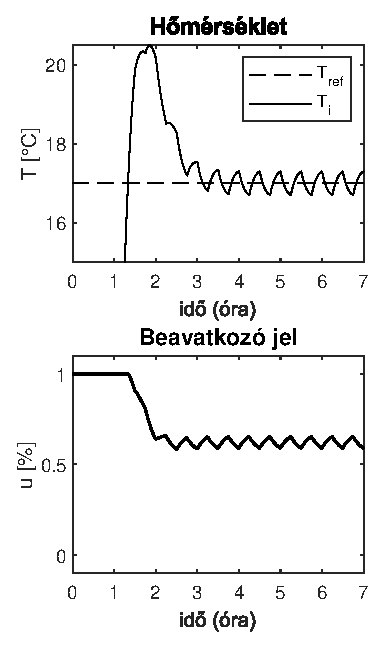
\includegraphics[width=\textwidth]{figures/realsys/mpc-wdu-100}
	\caption{$w_{\Delta u}=100$}
	\label{fig:mpc-wdu-100}
\end{subfigure}
~
\begin{subfigure}[t]{0.32\textwidth}
	\centering
	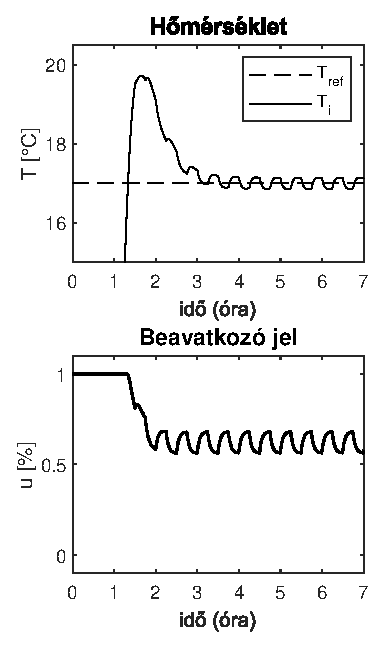
\includegraphics[width=\textwidth]{figures/realsys/mpc-wdu-50}
	\caption{$w_{\Delta u}=50$}
	\label{fig:mpc-wdu-50}
\end{subfigure}
~
\begin{subfigure}[t]{0.32\textwidth}
	\centering
	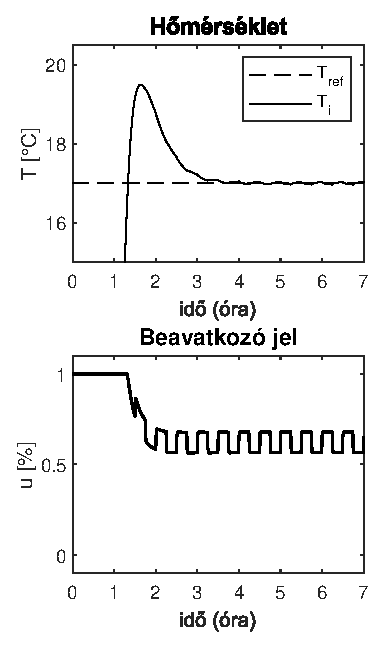
\includegraphics[width=\textwidth]{figures/realsys/mpc-wdu-10}
	\caption{$w_{\Delta u}=10$}
	\label{fig:mpc-wdu-10}
\end{subfigure}
\caption{MPC viselkedése  $w_{\Delta u}$ értékekre, $w_y=5$, $w_u=0.05$ mellett}
\label{fig:mpc-wdu}
\end{figure}





%% Feljesztési lehetőségek
%\begin{formal}
%	Még lehetséges:
%	\begin{itemize}[noitemsep,topsep=-8pt,parsep=0pt,partopsep=0pt]
%		%		\item kazán bekapcsolása
%		%		\item előremenő hőmérséklet - unmeasured VAGY uncontrolled inputként
%		%		\item 1 db. fűtőtest (most radiátor) szelepének tömegárama (szelep áteresztése)
%		%		\item Később több fűtőtest vagy többféle fűtőtestek (padlófűtés, különböző teljesítményű radiátorok) szabályozása
%		\item környezeti hőmérséklet: predikció / szekvencia használata% is lesz rá. Hatása a kimeneten már identifikálva lett, 3 pólussal és 2 zérussal tökéletesen lekövethető.
%		\item napsugárzás zavaró hatása% - szimulálható  a bizonytalansága valószínűleg nagy lesz
%	\end{itemize}
%	
%	Belső változók - fűtési rendszer és ház kapcsolata
%	\begin{itemize}[noitemsep,topsep=-6pt,parsep=0pt,partopsep=0pt]
%		\item napsugárzás - radiatív, az ablak felületével és a szöggel arányos
%		\item fűtőtestek sugárzó és konvektív hőárama
%	\end{itemize}
%	
%	Paraméterek a plantben nem állandók:
%	\begin{itemize}[noitemsep,topsep=-6pt,parsep=0pt,partopsep=0pt]
%		%		\item hőátadási tényezők hőmérsékletfüggők, áramlási sebesség-függők (szél)
%		\item szellőztetés, belső hőterhelés hatása
%	\end{itemize}
%\end{formal}